\documentclass[10pt,a4paper]{article}
\usepackage{geometry} 
\usepackage{graphicx}
\setlength\parindent{0pt}
\setlength{\parskip}{1em}
\usepackage{chngcntr}
\counterwithout{figure}{section}
\usepackage{amsmath} 

\title{Improving FASTBUS dead time by Event Switching}
\author{Mark Jones, Dasuni Adikaram}
%\date{} % delete this line to display the current date

%%% BEGIN DOCUMENT
\begin{document}

\maketitle
\tableofcontents

\section{Introduction}

The upcoming proton form factor experiment, GEp(5), measures the ratio of electric and magnetic elastic form factors of the proton at $Q^2$ up to $12$ GeV$^2$ via elastic electron-proton scattering. For electron detection, a large lead glass calorimeter (ECal) will be used with the Coordinate Detector (CDet). The proton will be detected in the SBS spectrometer which consist of front
tracker GEMs, a polarimeter and the hadron calorimeter (HCal). GEp(5) trigger has two levels: the level1 acceptance trigger (L1A) generated by the ECal, and the level 2 acceptance (L2A) trigger which is the coincidence between ECal and HCal. 

The conventional FASTBUS and VME electronics will be used for ECal. At high luminosity of $8\times10^{38}$ cm$^{-2}$s$^{-1}$, L1A rate is expected to be of the order of 200 KHz. This will result a FASTBUS front end dead time of about $40\%$, which is not acceptable. In order to reduce the front end dead time, the trigger can be passively split between two or three FASTBUS crates, so that when a crate is busy encoding, the next trigger will be sent to a non-busy crate eliminating the front end busy from the FASTBUS. The technique is called "event switching" and further details and its performance will be discussed in this report.

\section{Test setup}
Figure~\ref{fig:trig_ts} shows the test setup used to demonstrate the event switching principle. We used three FASTBUS (FB) crates, each with 8 ADCs ( LeCroy 1881M). The readout trigger was generated as follows: a radioactive source, Sr-90, was placed on the PMT-coupled scintillator and the analog PMT signal was discriminated to generate the readout trigger. We also used NIM random pulse generator (BNC DB-2) coupled with readout trigger to generate local trigger (Level 1 type trigger). 
\begin{figure}[ht]
\begin{center}
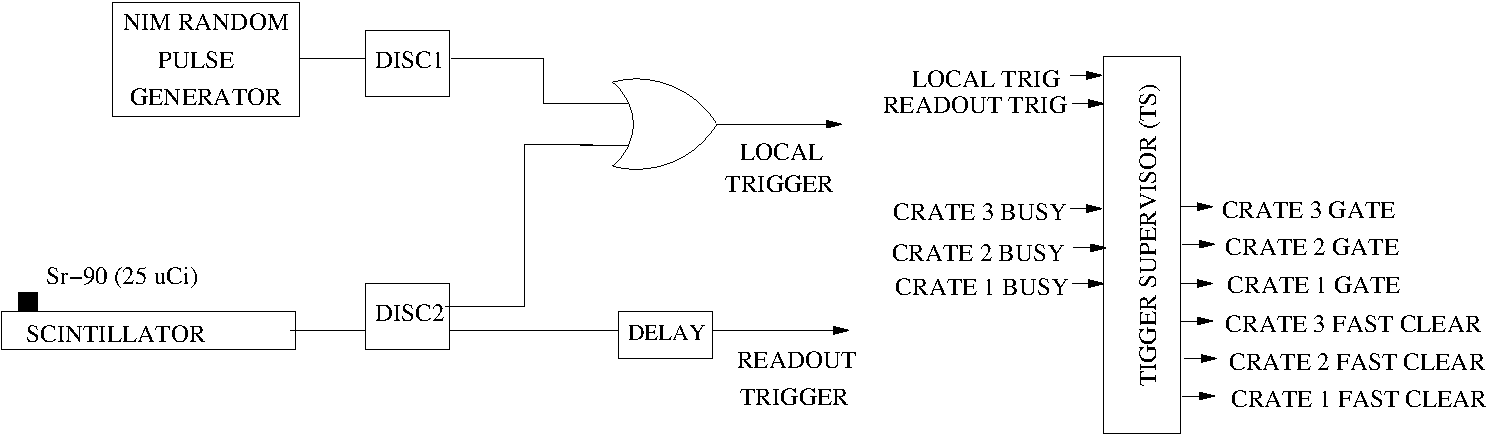
\includegraphics[width=0.9\textwidth]{Trigger_TS.pdf}\\
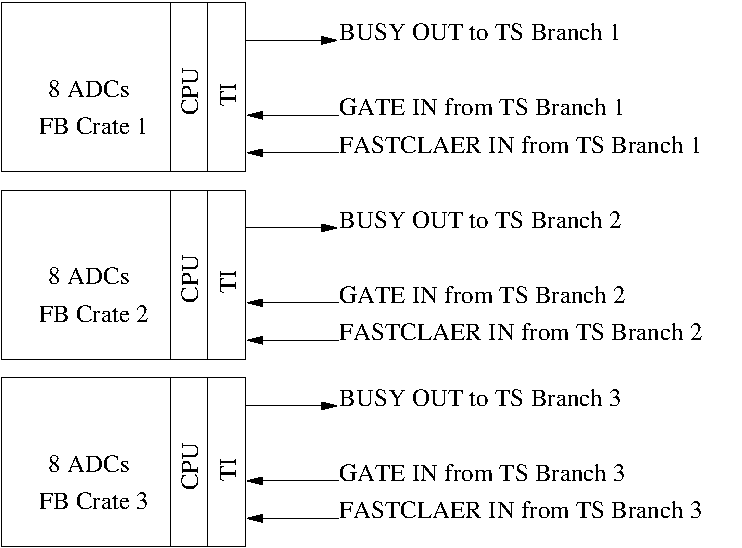
\includegraphics[width=0.5\textwidth]{FBCrates.pdf}
\end{center}
\caption{Test setup}
\label{fig:trig_ts}
\end{figure}

Note that the Readout trigger is a subset of the Local trigger, however, the Readout trigger may have a delay relative to Local trigger in FPGA due to the formation time of ECal and HCal coincidence. Local Trigger can be delayed up to $\sim2$ $\mu s$ in FPGA to match with readout trigger to generate "Fast Clear" or "Not Fast Clear" signal. During the test, we delayed the Readout trigger by $\sim744$ ns and the latency of the Local trigger was set to $756$ ns (VME register offset 0x118 bits(18:10)), so that the Readout and Local triggers are within a \textit{40 ns veto window}, which is a necessary requirement in this TS design ( see Figure~\ref{fig:fc_scope}).

The readout trigger was varied between 500 Hz - 10 kHz, and the local trigger was varied between 10kHz - 200 kHz during the test. In order to keep the Local trigger rate at  a constant value while varying the Readout trigger rate (varying the discriminator-DISC1 threshold level), we have to adjust the discriminator-DISC2 threshold level accordingly. Readout and local trigger were send to SBS trigger supervisor. 
 
\subsection{SBS Trigger Supervisor (TS)}
The TS acts as the central control point for data acquisition. The trigger/clock/sync signals from TS pass to the Signal Distribution (SD). SD can fan out the signals to (up to) 16 Trigger Distribution (TD) modules and TD can fan out to (up to) eight Trigger Interface (TI) modules in FB crates via optical transceivers. The busy signals from front end electronics can propagate back to the TS in the other direction.  Figure~\ref{fig:ts} shows the block diagram of the TS module used in the test including its major components. Main features of TS can be summarized as below. 
\begin{figure}[ht]
\begin{center}
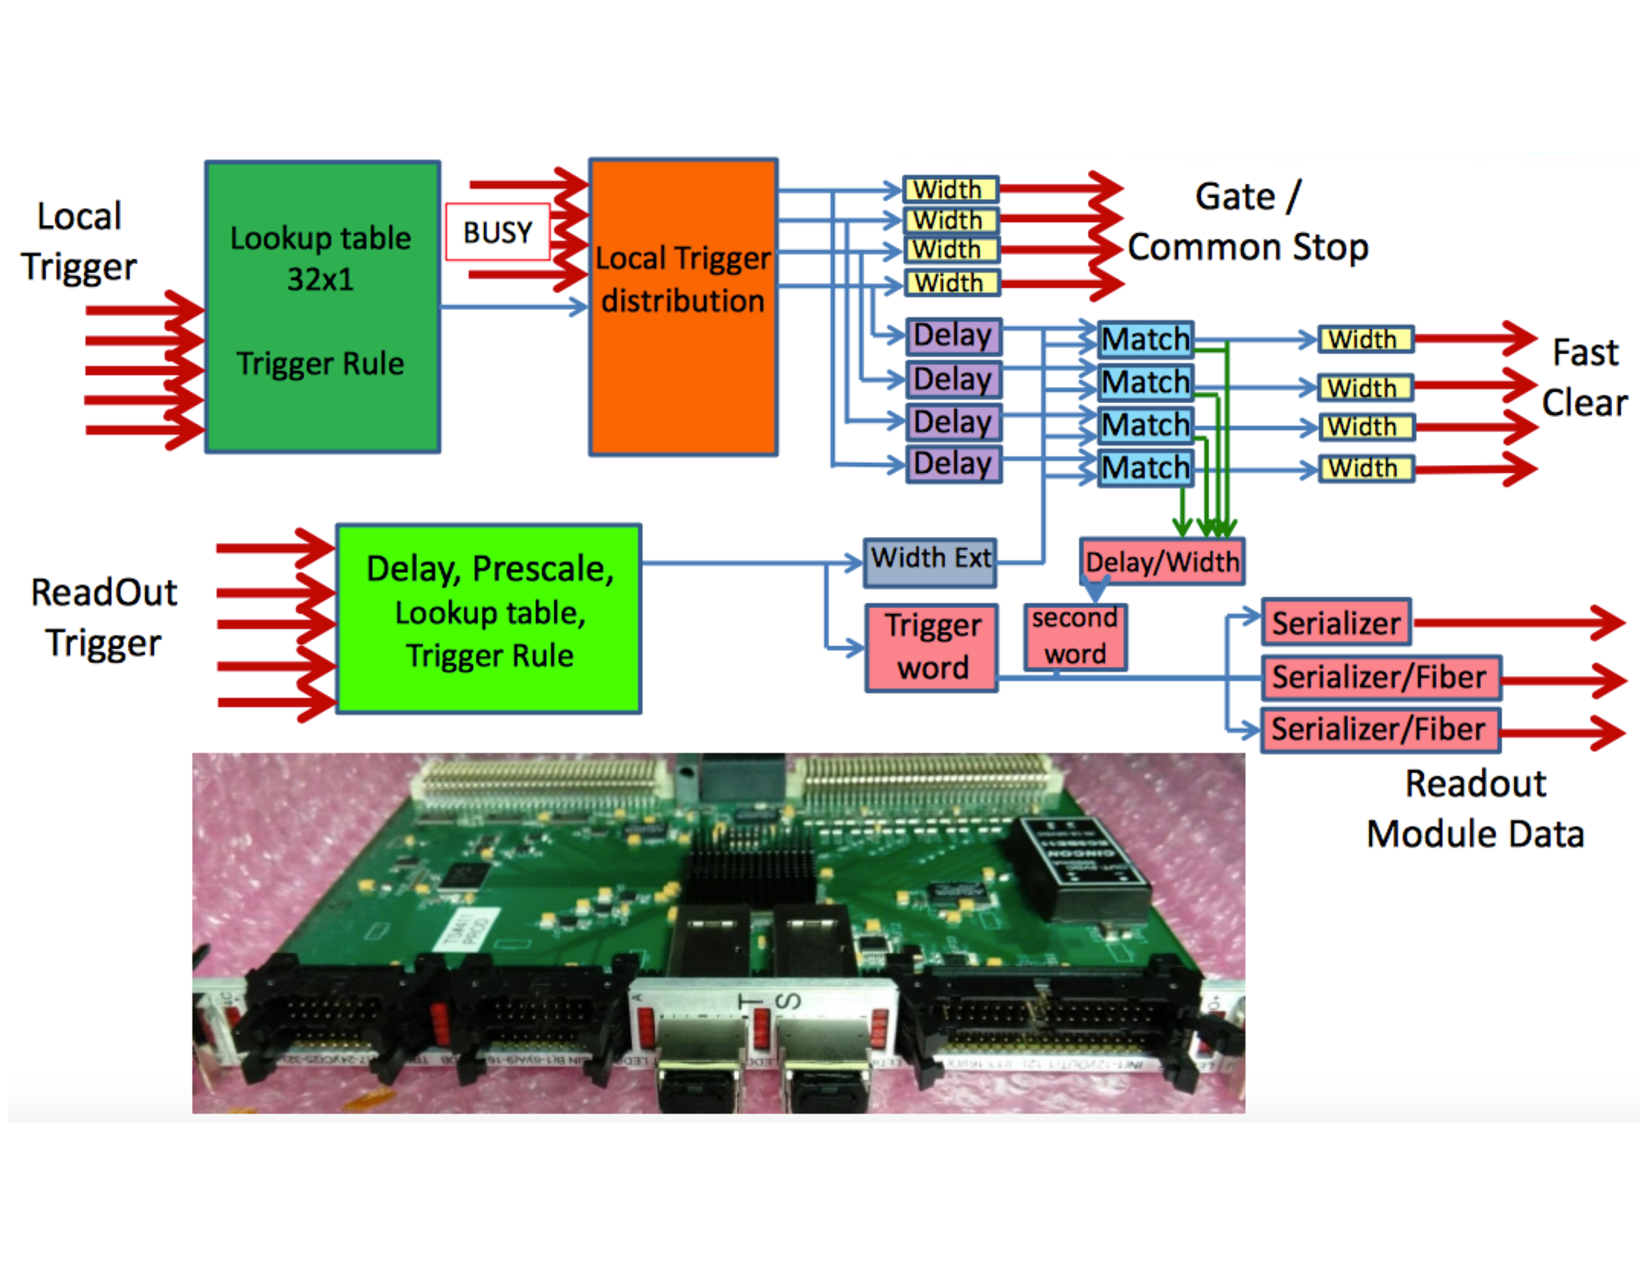
\includegraphics[width=0.95\textwidth]{TS.pdf}
\end{center}
\caption{Functional diagram of SBS Trigger Supervisor (TS)}
\label{fig:ts}
\end{figure}

\begin{itemize}
\item We can use up to five local trigger inputs to generates the local trigger. A simple rule is applied to the Local Trigger, so that the same event will not be readout twice. The rule is: there is no more than ONE local trigger in time $T$. The time $T$ is set register 0x70, bit (6:0) in 4 ns steps. During the test, $T$ was set to 128 ns. \textit{Note that if the local trigger width is wider than the local trigger rule, then it will generate a second trigger after trigger rule expires. This means that the third (or more) trigger is possible for wider local trigger inputs.} 

The Local Trigger can be distributed to (up to) four duplication branches, each links to one FB crate, in round-robin manner. The front end can assert a BUSY signal, and the BUSY will propagate to the TS. If one branch is BUSY, TS will automatically skip that branch and look for the next non-BUSY branch. The register offset 0x28 bit(15-12) is used to set the available DAQ duplication branches. The Local Trigger signal width can be set using register offset 0x70, bit(15:8) in steps of 4 ns. Local trigger width was set to 128 ns during the test. Once TS receives a Local trigger, it sends a ADC gate signal to the next non-BUSY crate. The width of the gate signal is $\sim140$ ns (Figure~\ref{fig:fc_scope}).

\item The readout trigger is common for all branches and it can be delayed due to the formation time of ECal and HCal coincidence as mentioned earlier. The readout trigger collisions happen when two or more event readout triggers are needed to send in the same time window (16 ns), or the front end electronics is busy, or the trigger is inhibited. If the trigger collision happens, the trigger will be lost. The TS will record it as busy time.

\item TS sends Fast Clear signal to abort the ADC conversion and thus minimizes the front end dead time. There are four Fast Clear signals corresponding to the four duplication branches. The Fast Clear signal is delayed Local trigger vetoed by the Readout trigger. The Fast Clear latency is set by VME register offset 0x118 bits(18:10) in 4 ns steps. The Fast Clear signal width can be set by register offset 0x70, bits(23:16) in 4 ns steps. During the test, Fast Clear latency was set to 756 ns and the Fast Clear signal width was set to 400 ns (see Figure~\ref{fig:fc_scope}).
\begin{figure}[]
\begin{center}
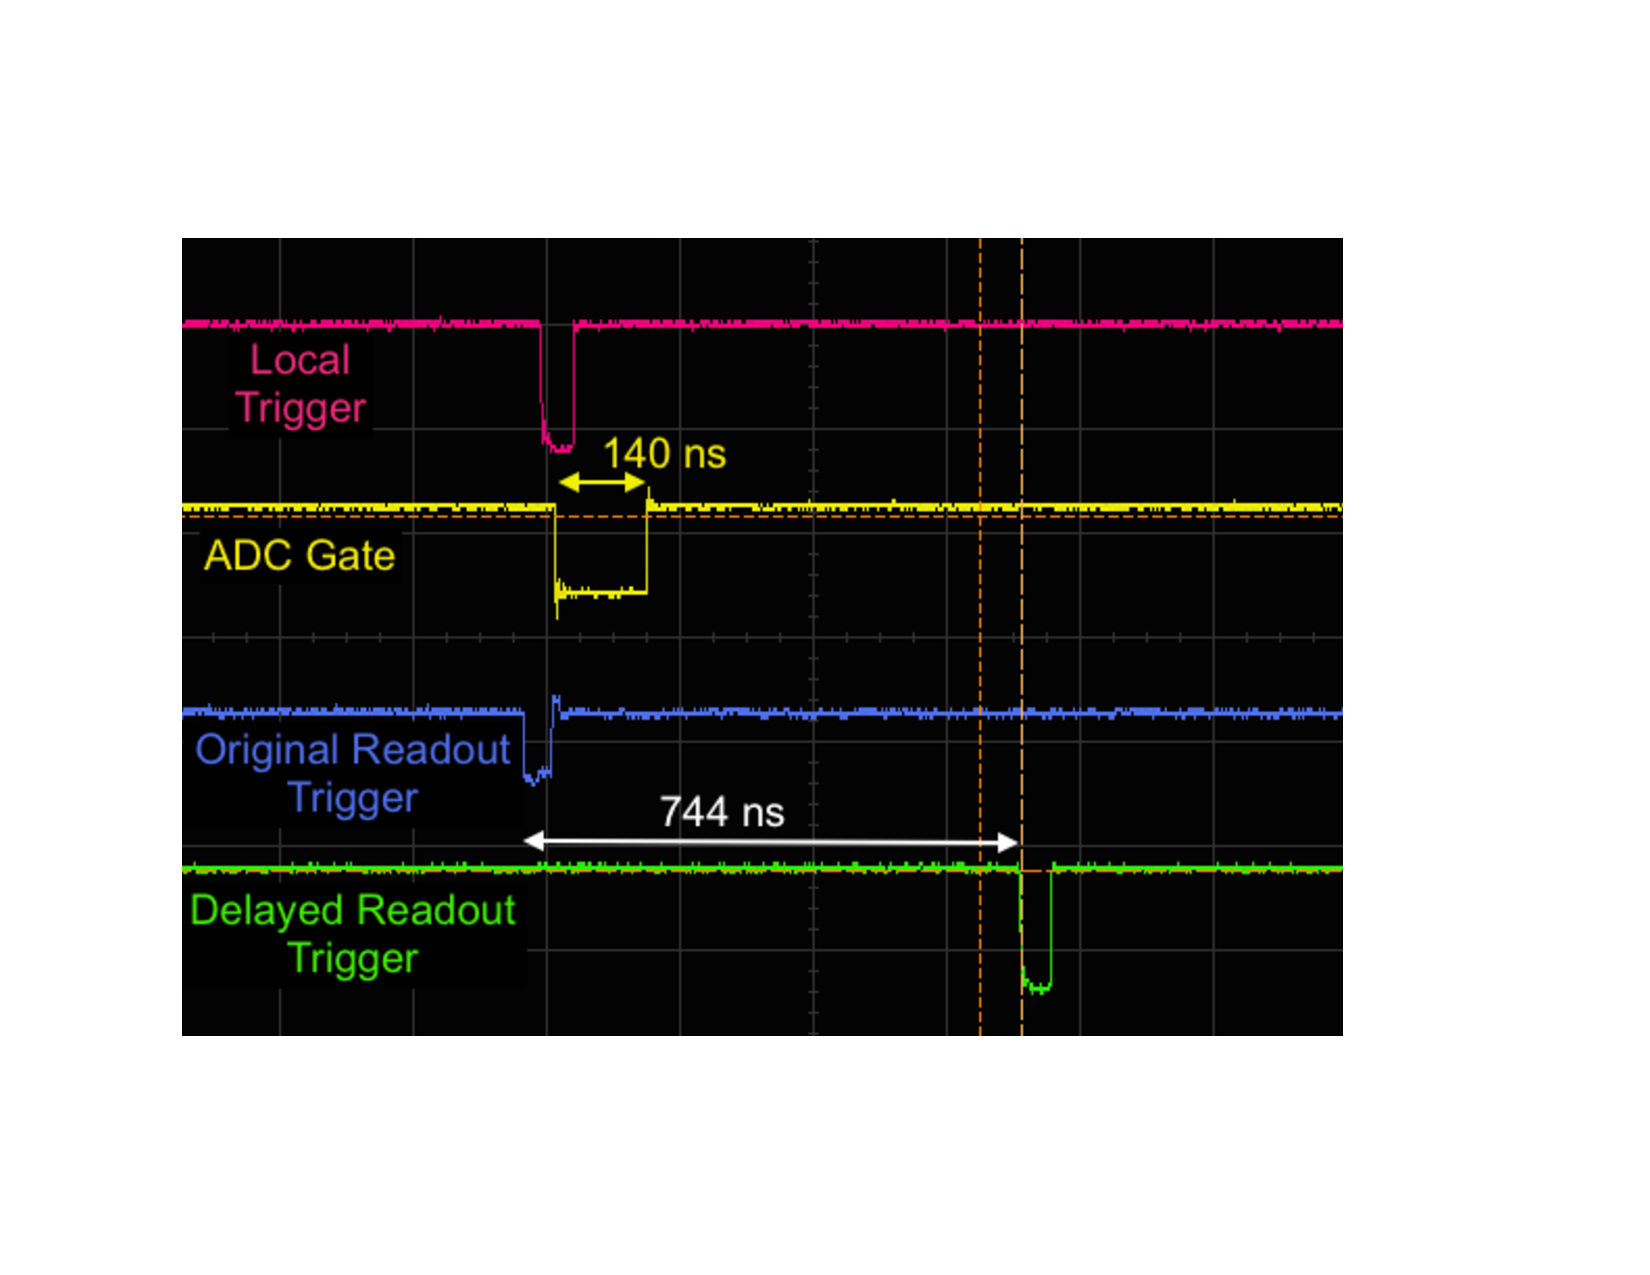
\includegraphics[width=0.405\textwidth]{scope_2.pdf}
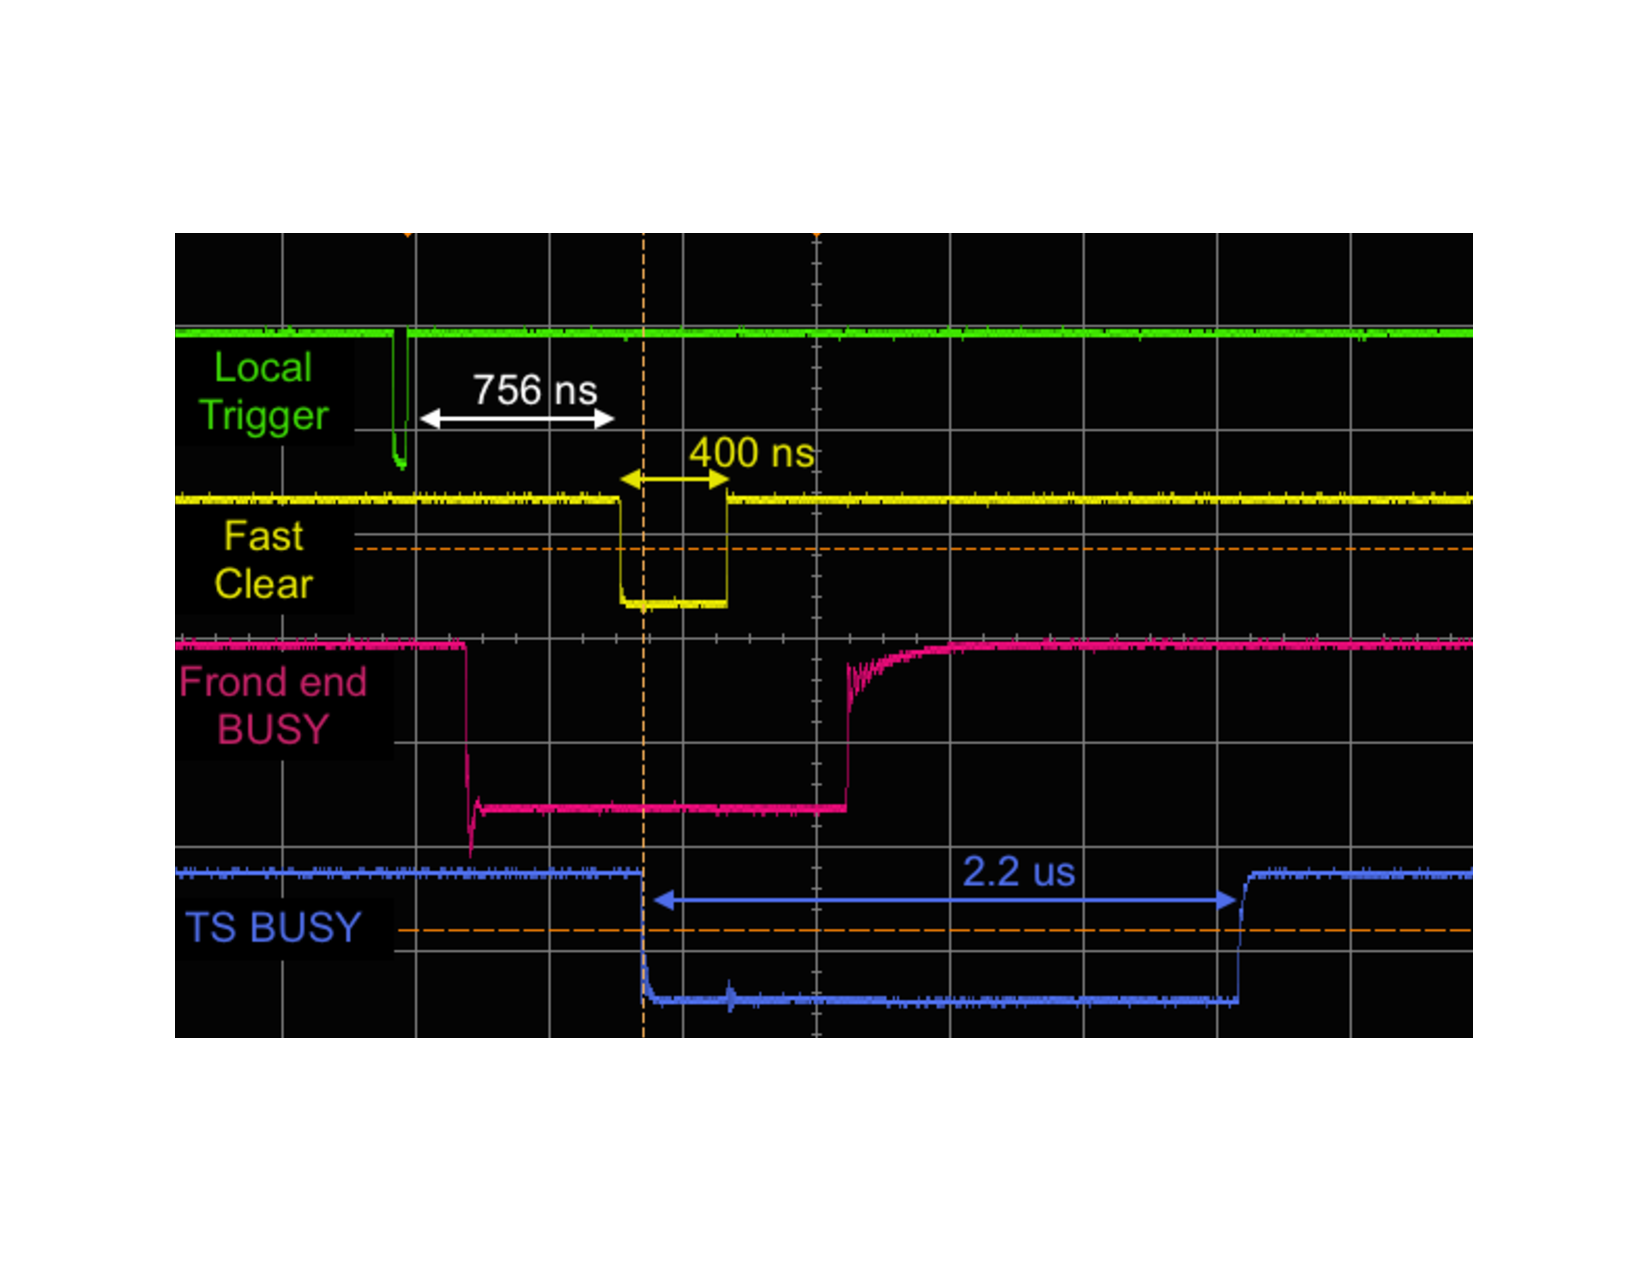
\includegraphics[width=0.45\textwidth]{FC_scope.pdf}
\end{center}
\caption{Oscilloscope output showing the timing for Local, Readout and ADC Gate for a readout event (left) and the timing for a fast cleared events (right).}
\label{fig:fc_scope}
\end{figure}
Upon ReadOut trigger, a window will be open to veto the Fast Clear so that the DAQ boards can save the digitized data and be read out. The veto window size is set by the VME register offset 0x70, bits(31:24) in 4 ns steps. Fast Clear veto width was set to 200 ns, during the test.
\end{itemize}

\section{Test Performance}
\subsection{Non-buffered mode}
In non-buffered mode, TS is able to accept new triggers only when the previous event has been completely read out. 
\subsubsection{Single Ctare}
In single crate operation, the total dead time of the FB system is caused by 2 ways (see Figure~\ref{fig:single_crate_timing}). 
\begin{itemize}
%\item Frond end Busy ($dt_{FE}$): Also called ``conversion dead time". It occurs following each Readout trigger when the ADCs are converting analog signals into digital format. If front end busy asserts, the system is unable to accept new data. It can be measured from the FB backplane and for 1881M ADC, $dt_{FE} \sim 8.5 \mu s$.
\item Readout Busy ($dt_{R}$): If the event is accepted, DAQ system is dead for some period to read that event out. No other events (except for remains buffer events) will be accepted during that time. For a FB crate in our setup (while reading pedestals of 6 channels of each ADC), $dt_{R} \sim 60 - 80 \mu s$. 
\item Fast Clear ($dt_{FC}$): If there is a local trigger, but no readout trigger, then TS issues a CLEAR signal to the front end modules to minimize the dead time of the system. Following a Local trigger, there is a dead period in TS until the Readout trigger or Fast Clear is issued. TS busy time for the fast cleared events can be set by changing the VME register settings and it was set to $dt_{FC} \sim 2.2 \mu s$ during the test (see Figure~\ref{fig:fc_scope}).
\end{itemize}

\begin{figure}[]
\begin{center}
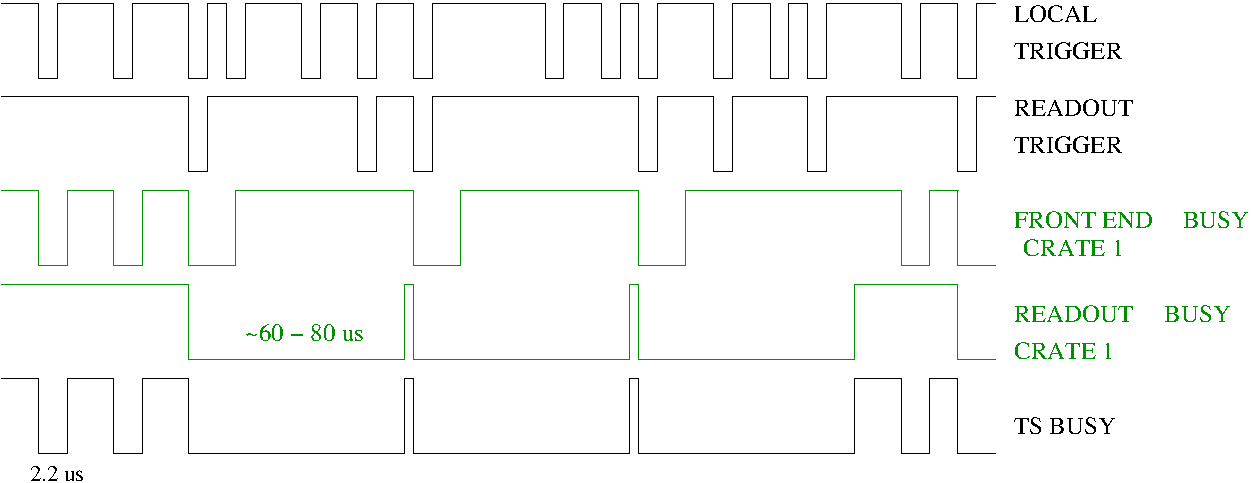
\includegraphics[width=0.75\textwidth]{single_crate_FC.pdf}
\end{center}
\caption{Timing diagram for single crate at non-buffered mode (BUFFER LEVEL = 1).}
\label{fig:single_crate_timing}
\end{figure}

\textbf{Dead time Model}\\
Dead times are typically modelled as being of two varieties: 
\begin{itemize}
\item Non-extendable, or non-paralyzable dead times are those in which events with an interarrival period of less than the dead time of the server,$\tau$, are lost and have no other effect on the server. 
\item Extendable, or paralyzable dead times are those in which the arrival of a subsequent event during a dead time period extends the dead time of the server from the time of the second event�s arrival by another period,$\tau$. This causes a prolonged period during which the events subsequent to the first are not recognized.
\end{itemize}
Assuming the time to process one event is $\tau$ and triggers are being generated at the average random rate $f$ , the dead time of a non-extendable system can be given as
\begin{equation}
DT = \frac{f\tau}{f\tau+1}
\end{equation}
For the non-extendable system, it can be given as
\begin{equation}
DT = \sum_{n=1}^{\infty} \frac{\mu^n e^{-\mu}}{n\ !}
\end{equation}
where $\mu = f\tau$.

Thus, during the non-buffered mode, the dead time contribution due to the readout can be written as
\begin{equation}
DT_R = \frac{\mathrm{L2}dt_R}{\mathrm{L2}dt_R+1}
\end{equation}
where L2 is the average readout trigger rate. When the Local trigger rate is equal to the Readout trigger rate, the total dead time, $DT = DT_R$.

When the Local trigger rate is greater than the Readout trigger rate, the contribution from the fast cleared events needs to be taken in to account.
\begin{equation}
DT_{FC} = \frac{(\mathrm{L1} - \mathrm{L2})dt_{FC}}{(\mathrm{L1} - \mathrm{L2})dt_R+1}
\end{equation}
where $\mu_{FC} = (L1-L2).dt_{FC}$ and L1 is the average local trigger rate. So, the total dead time of the non-buffered system can be written as,
\begin{equation}
DT = DT_{R} +  DT_{FC} - DT_{R}\times DT_{FC}
\end{equation}

\subsubsection{Event switching}

\begin{figure}[]
\begin{center}
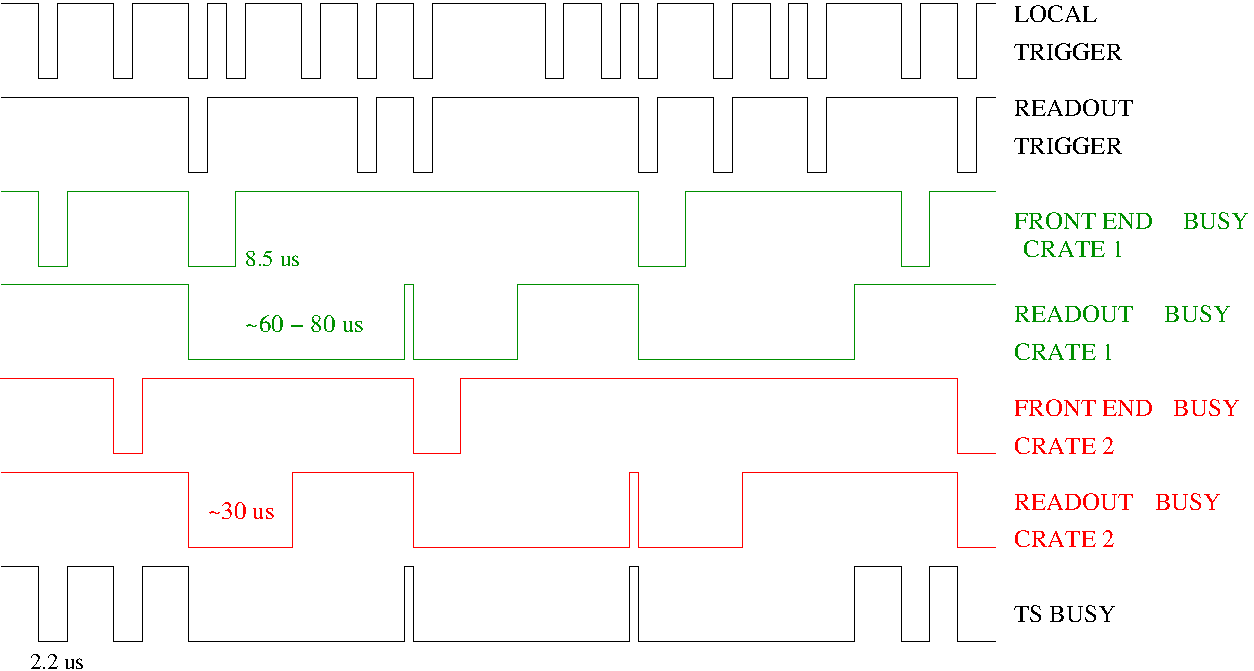
\includegraphics[width=0.75\textwidth]{buff1_switching.pdf}
\end{center}
\caption{Timing diagram for event switching at non-buffered mode (BUFFER LEVEL = 1).}
\label{fig:swithing_timing}
\end{figure}

Timing diagram for the event switching at non-buffer mode is shown in Figure~\ref{fig:swithing_timing}. When the trigger is switching between multiple crates, dead time due to a fast cleared event only occurs if all $n$ crates are busy. Therefore, we use $DT_{FC} = (DT_{FC})^n$, where $n$ is the number of FB crates used in the system. There is also a busy time of $\sim30$ $\mu$s on the other crates which do not process the event readout. It is because we are currently reading out some of the TI data, i.e. TI data is used to identify which FB duplication branch has data and the event will be broadcast by the front-end modules only if the event is sent to the corresponding branch. However, this $\sim30$ $\mu$s busy time cause no additional dead time on the system in this configuration since it occurs simultaneously with $dt_R \sim60\mu$s.

\begin{figure}[]
\begin{center}
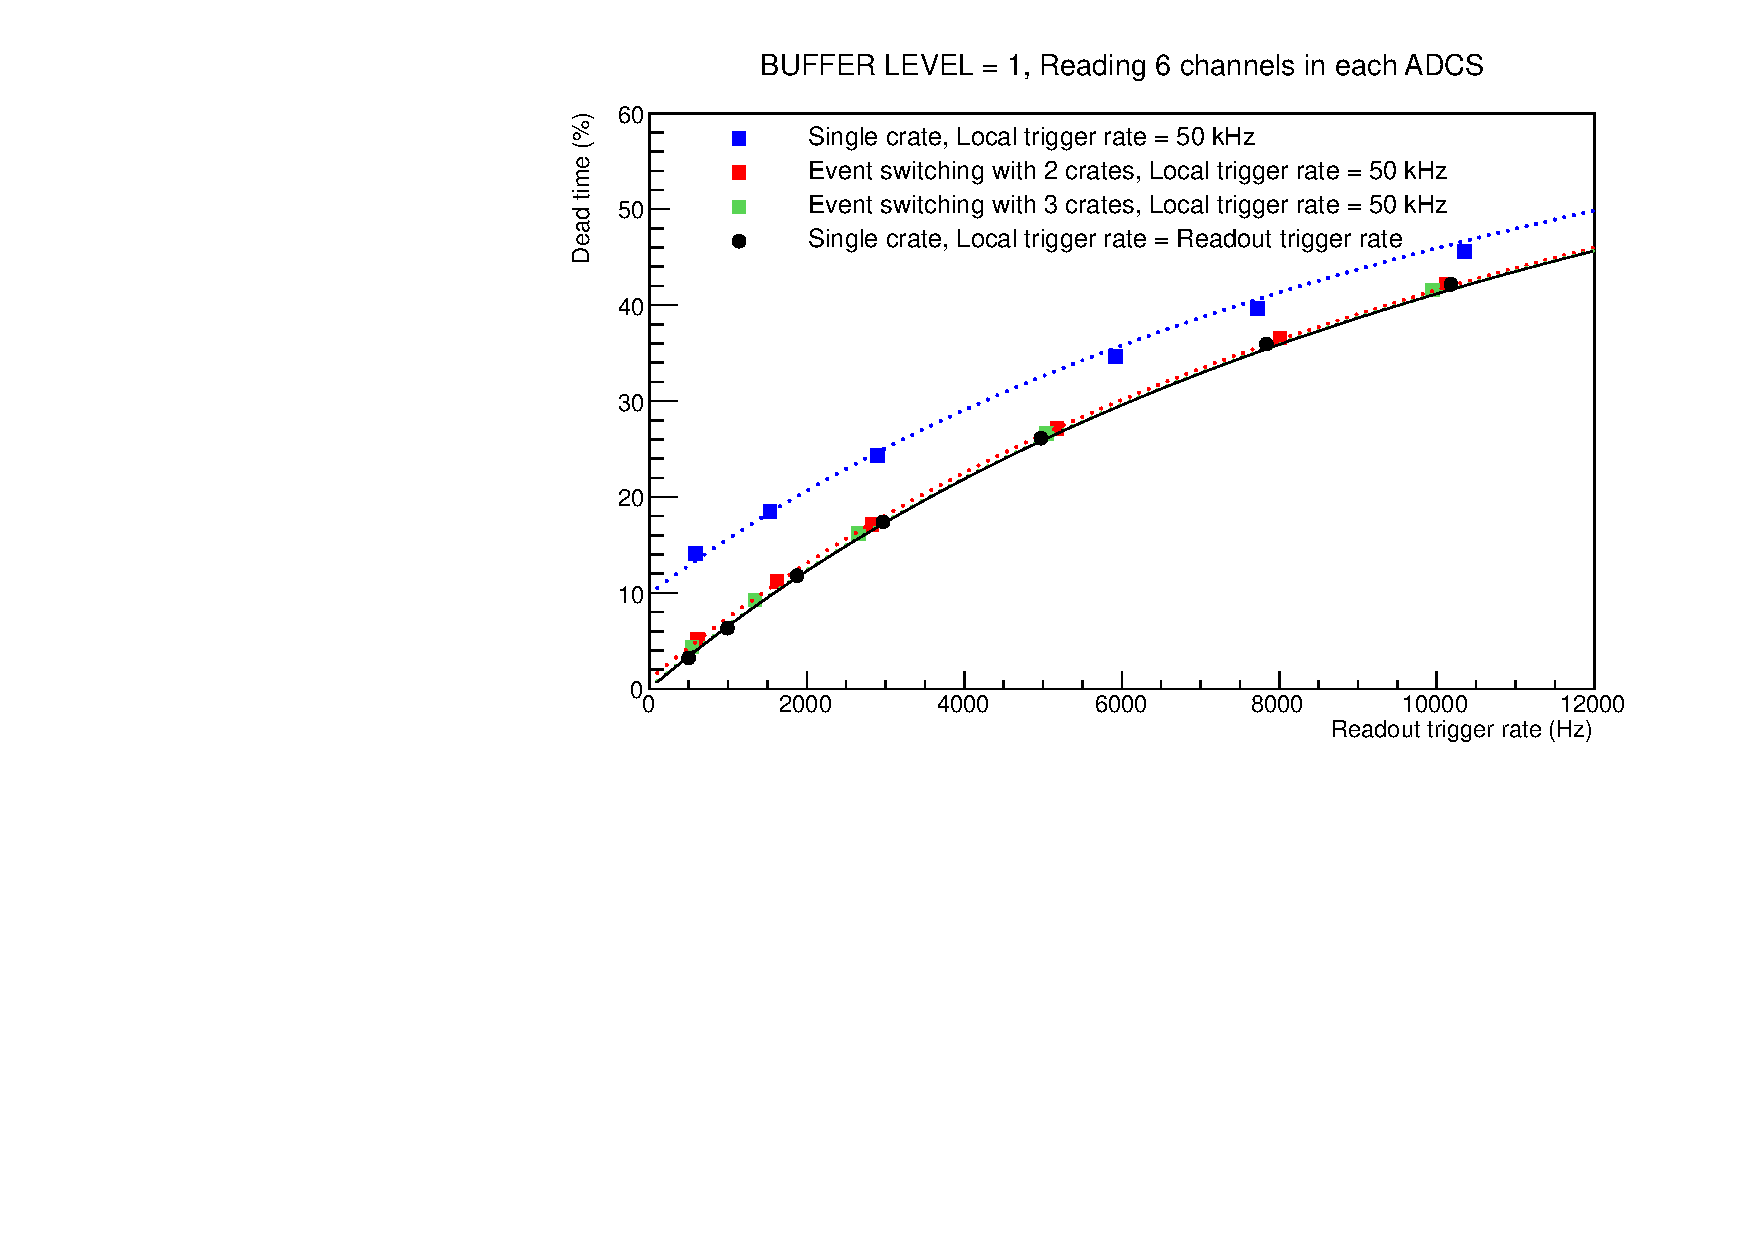
\includegraphics[width=0.75\textwidth]{diffCrate_buffer_1_Local_50k_v4.pdf}
\end{center}
\caption{Measured dead time as function of readout trigger rate at BUFFER LEVEL = 1. The black solid line (data) represents the dead time calculated by the model (measured) when Local trigger rate = Readout trigger rate. The colored dotted-lines (data) represent the dead time calculated by the model (measured) at Local trigger rate = 50 kHz with different number of FB crates.}
\label{fig:diffCrate_buf1}
\end{figure}

As shown in Figure~\ref{fig:diffCrate_buf1}, switching the input trigger between multiple crate is not very effective at non-buffered mode as expected. The dead time due to the events being read out is same for single crate and event switching modes. There is only a slight improvement in the dead time when the Local trigger rate is large compared to the Readout trigger rates, because the fast cleared events are switching between the multiple crates. 

Figure~\ref{fig:diffChannel_buf1} shows how the dead time of a non-buffered single crate varies as the number of channels reading in each ADC increases. From the oscilloscope, we observed that $dt_{R} = 60 - 80$ $\mu s$ when reading only 6 channels in each ADC, $dt_{R} = 110 -130$ $\mu s$ when reading 32 channels in each ADC and $dt_{R} = 160 - 180$ $\mu s$ when reading all channels in all 8 ADCs. The total dead time of the FB system also increases with number of ADC channels reading in as expected. 
\begin{figure}[]
\begin{center}
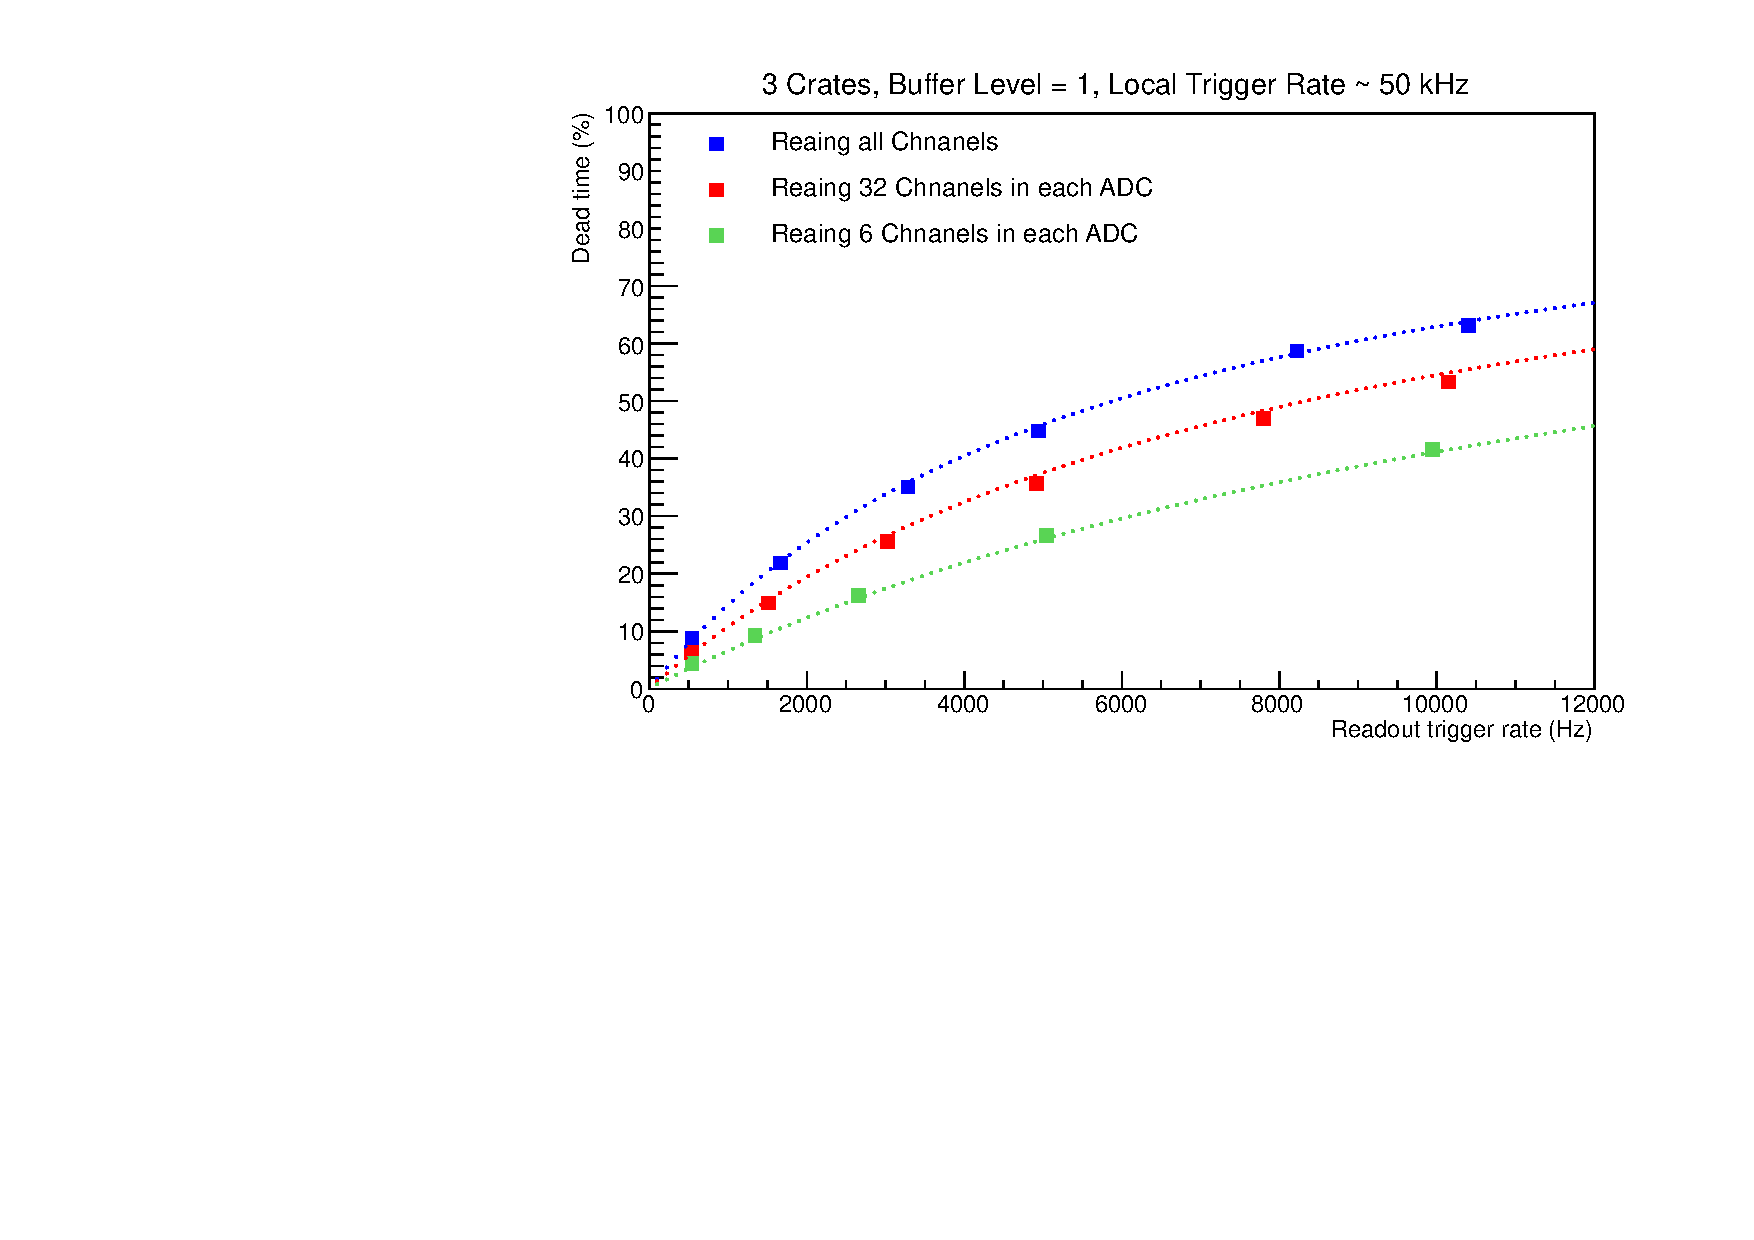
\includegraphics[width=0.75\textwidth]{diffChannels_buffer_1_local_50k.pdf}
\end{center}
\caption{Measured dead time as function of readout trigger rate at BUFFER LEVEL = 1 for a single crate. The colored dotted-lines (data) represent the dead time calculated by the model (measured) at Local trigger rate = 50 kHz when reading different number of channels in ADCs (LeCroy 1881M).}
\label{fig:diffChannel_buf1}
\end{figure}

\subsection{Buffered mode}
When TS is used in buffered mode, it can process a new event while reading out previous event. The number of events processes at a time is defined as the depth of the buffer (or BUFFER LEVEL). 

\subsubsection{Single Crate}
Figure~\ref{fig:single_crate_timing_diffbuf} shows the timing diagram for a single crate when the depth of the TS branch buffer is set to 4. Now, the readout will only contribute to the dead time if the 4-deep trigger buffer gets full. Then an event must be completely read out of the front-end modules to allow space for the next trigger. Having onboard buffering decouples the readout dead time from the front end dead time, allowing a properly integrated system to run as fast as the front end operation permits.

\begin{figure}[]
\begin{center}
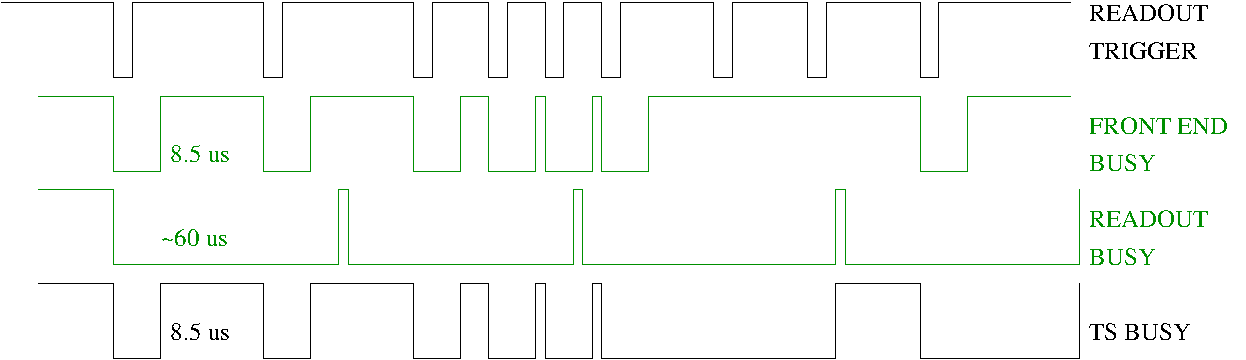
\includegraphics[width=0.75\textwidth]{single_crate_buff4.pdf}
\end{center}
\caption{Timing diagram for single crate at BUFFER LEVEL = 4.}
\label{fig:single_crate_timing_diffbuf}
\end{figure}

Since the readout dead time is now contribute to the system only when the buffer is full, the readout dead time component for the buffered mode can be written as
\begin{equation}
DT_{R} = \sum_{n=b}^{\infty} \frac{\mu_{R}^n e^{-\mu_{R}}}{n\ !}
\end{equation}
where $b$ is the depth of the buffer and $\mu_{R} = L2.dt_{R}$.
The decoupling between front end busy and readout busy introduces a new component to the dead time due to the front end busy and it can be defined as
\begin{equation}
DT_{FE} = \sum_{n=1}^{\infty} \frac{\mu_{FE}^n e^{-\mu_{FE}}}{n\ !}
\end{equation}
where $\mu_{FE} = L2.dt_{FE}$, and $dt_{FE} \sim 8.5$ $\mu \mathrm{s}$. Thus, the total dead time of the system can be written as
\begin{eqnarray}
DT = DT_{R}(1- DT_{FC} - DT_{FE}) &+& DT_{FC}(1- DT_{R} - DT_{FE}) \nonumber \\
&+& DT_{FE}(1- DT_{R} - DT_{FC})
\end{eqnarray}

\begin{figure}[]
\begin{center}
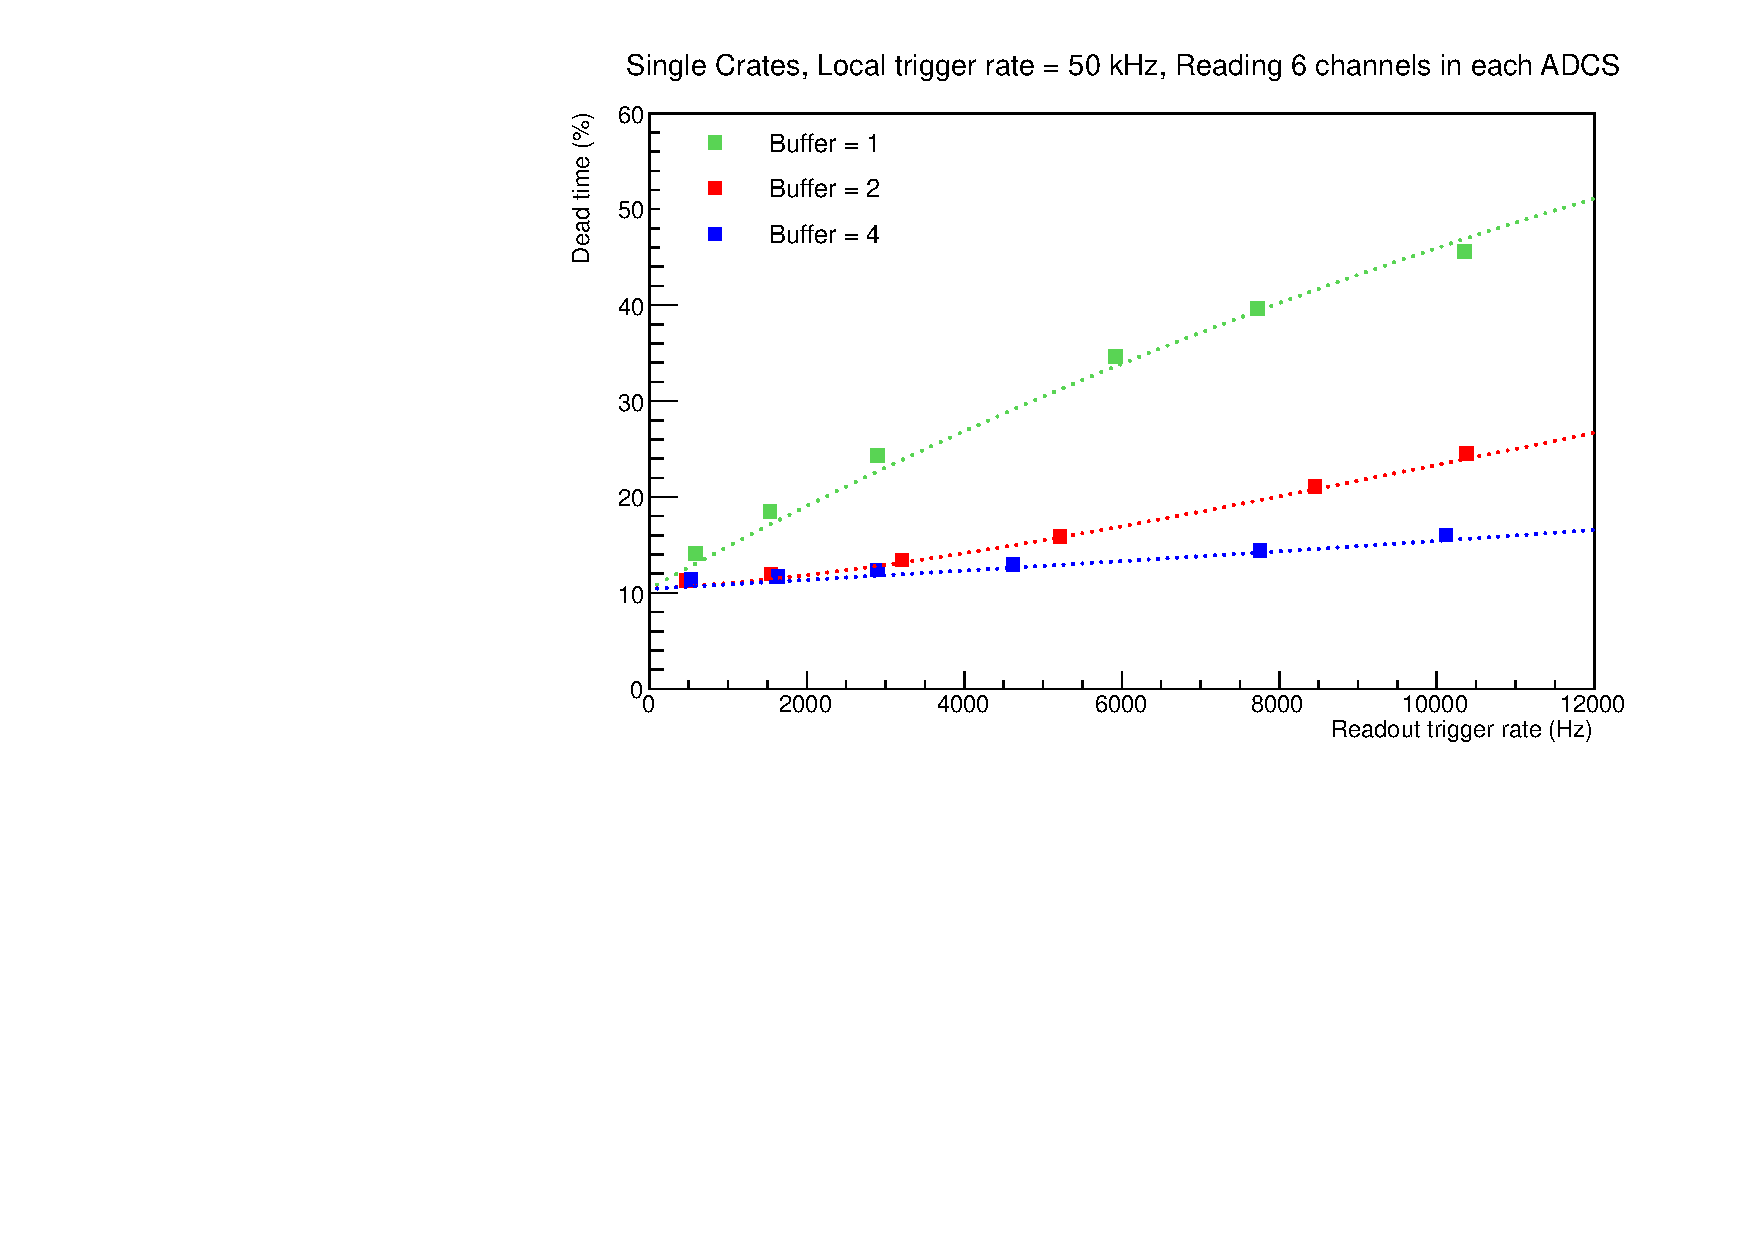
\includegraphics[width=0.75\textwidth]{singleCrate_diffBuffer_Local_50k.pdf}
\end{center}
\caption{Measured dead time as a function of Readout trigger rate with different depths of buffer. The colored dotted-lines (data) represent the dead time calculated by the model (measured) at Local trigger rate = 50 kHz with different buffer depths and a single FB crate.}
\label{fig:singleCrate_diffbuf}
\end{figure}

Figure~\ref{fig:singleCrate_diffbuf} shows the measured dead time for a single FB crate system with different depths of TS buffer along with calculated dead time by the model. It can be clearly seen that, at the high Local trigger rate of 50kHz, additional buffers make a very modest improvement in the dead time. At Readout trigger rate = 10kHz, the improvement is about factor of 4 if the depth of the buffer is increased from 1 to 4.

\subsubsection{Event Switching}

The operation of event switching mode at BUFFER LEVEL = 4 is illustrated in Figure~\ref{fig:switching_timing}. Once an event send to a non-BUSY crate, TS no longer remains busy until the corresponding frond end busy is get cleared. Instead TS undergo a short busy of 128 ns, and then TS is ready to accept another readout trigger. BUSY signals from the three crates propagate to the TS, so the next event will be sent to the next non-BUSY crate. Once the TS buffer is full, TS remains busy until one of the events in the buffer being readout. Once an event read out completely, TS is again ready to accept another readout trigger. Note that in current test setup, when one FB crate is reading out an event, the other crate/crates is/are also busy for about $\sim$30 $\mu s$.

\begin{figure}[]
\begin{center}
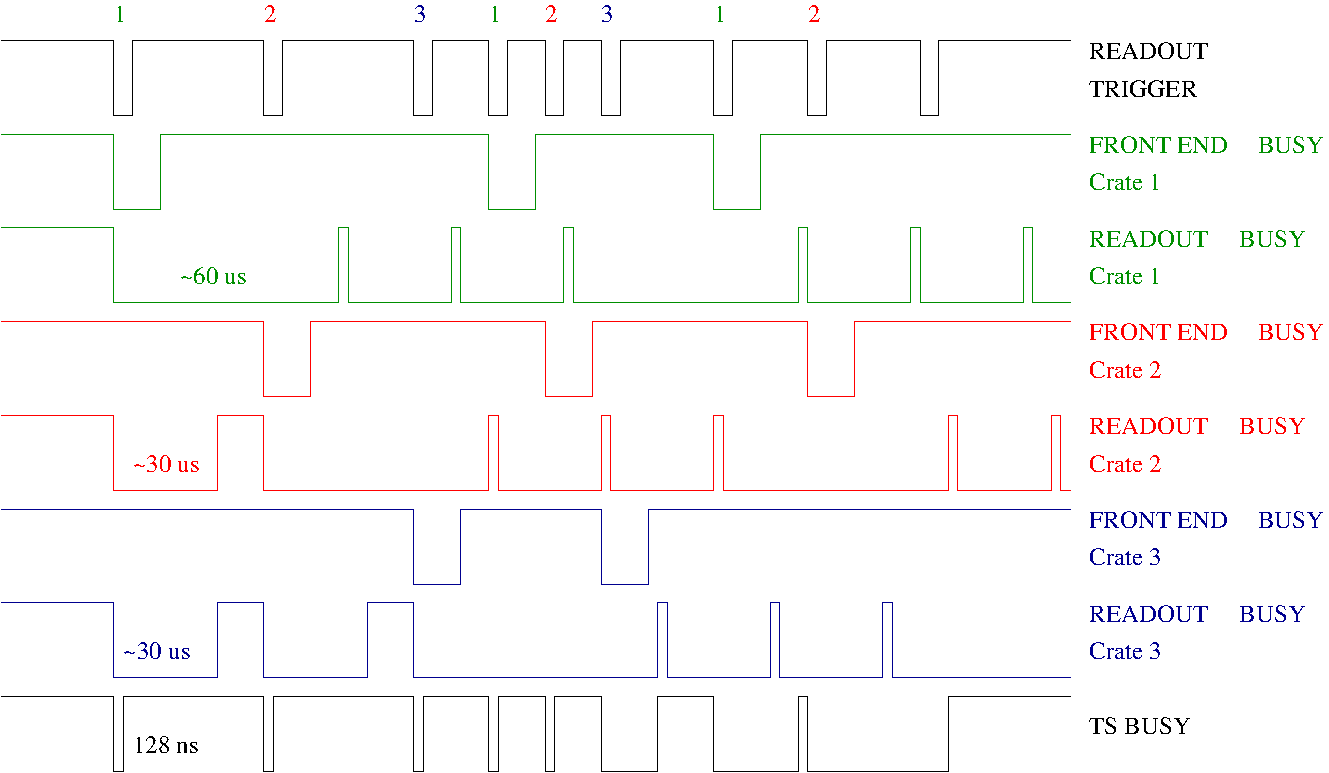
\includegraphics[width=0.75\textwidth]{single_crate_buff4_switching.pdf}
\end{center}
\caption{Timing diagram for event switching with three FB crates at BUFFER LEVEL = 4.}
\label{fig:switching_timing}
\end{figure}

This additional $30$ $\mu s$ also makes a contribution to the total dead time, especially at higher Readout trigger rates. In order take that into account, we use following steps.

The dead time due to the readout busy time in the FB crate which processes the readout, 
\begin{equation}
DT_{R1} = \sum_{n=b}^{\infty} \frac{\mu_{R1}^n e^{-\mu_{R1}}}{n\ !}\nonumber
\end{equation}
where $\mu_{R1} = L2.dt_{R}$ and $dt_R\sim60$ $\mu s$. The dead time due to the additional readout busy time occurs in the other crates,
\begin{equation}
DT_{R2} = \sum_{n=b}^{\infty} \frac{\mu_{R2}^n e^{-\mu_{R2}}}{n\ !}\nonumber
\end{equation}
where $\mu_{R2} = L2.dt_{R2}$ and $dt_{R2}\sim30$ $\mu s$. Then we combine these contributions to obtain the total dead time due to the readout busy time,
\begin{equation}
DT_{R} = DT_{R1} (1- DT_{R1}) + DT_{R2} (1- DT_{R1})
\end{equation}

Also, the dead time contribution of front end busy time needs to be replaced by short busy time of TS ($128$ ns),
\begin{equation}
DT_{TS} = \sum_{n=1}^{\infty} \frac{\mu_{TS}^n e^{-\mu_{TS}}}{n\ !}
\end{equation}
where $\mu_{TS} = L2.dt_{TS}$ and $dt_{TS} \sim 128$ ns. Thus, the total dead time of the system can be written as
\begin{eqnarray}
DT = DT_{R}(1- DT_{FC} - DT_{TS}) &+& DT_{FC}(1- DT_{R} - DT_{TS}) \nonumber \\
&+& DT_{TS}(1- DT_{R} - DT_{FC})
\end{eqnarray}

\begin{figure}[]
\begin{center}
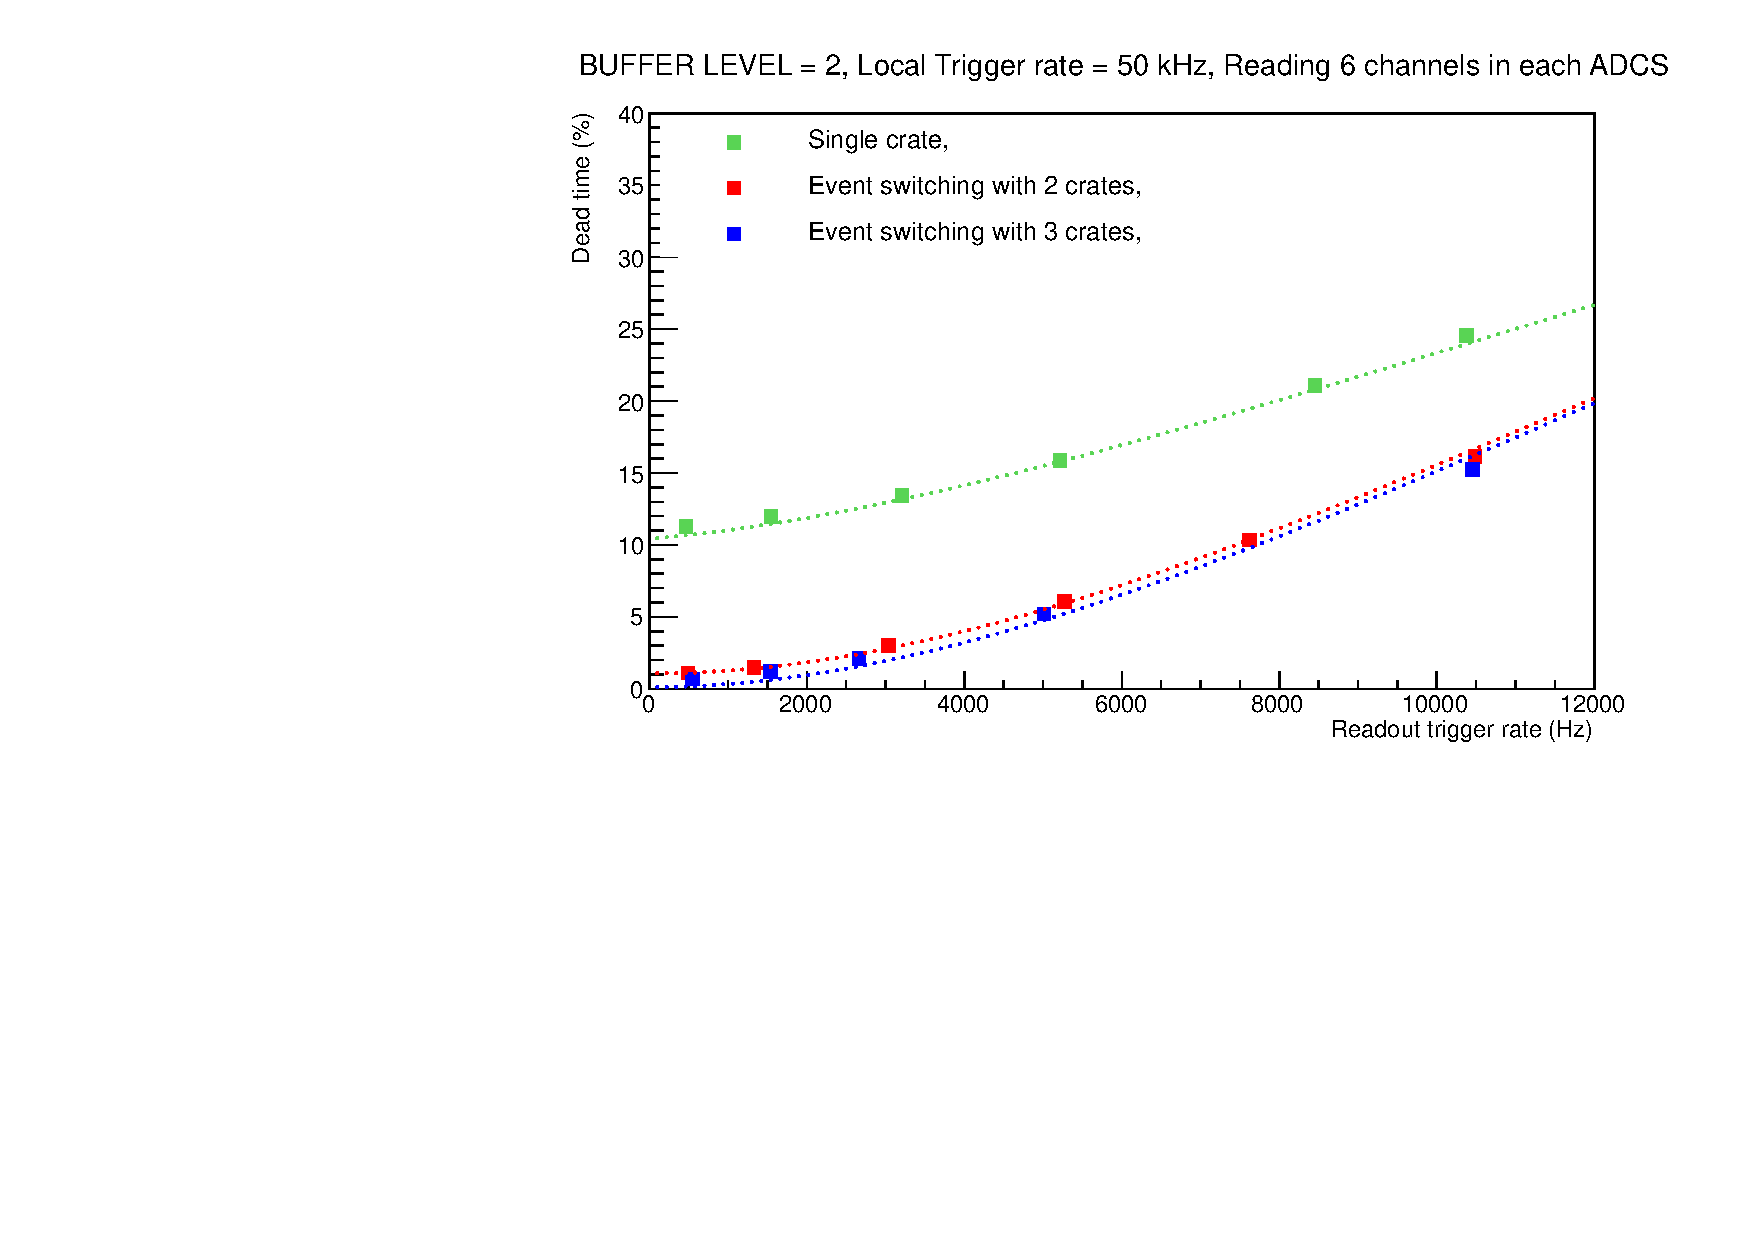
\includegraphics[width=0.75\textwidth]{diffCrate_buffer_2_Local_50k.pdf}
\end{center}
\caption{Dead time comparison of a single crate system and the event switching mode at Local trigger rate = 50 kHz. The colored dotted-lines (data) represent the dead time calculated by the model (measured) at BUFFER LEVEL = 2.}
\label{fig:diffCrate_buf2_local_50}
\end{figure}

\begin{figure}[]
\begin{center}
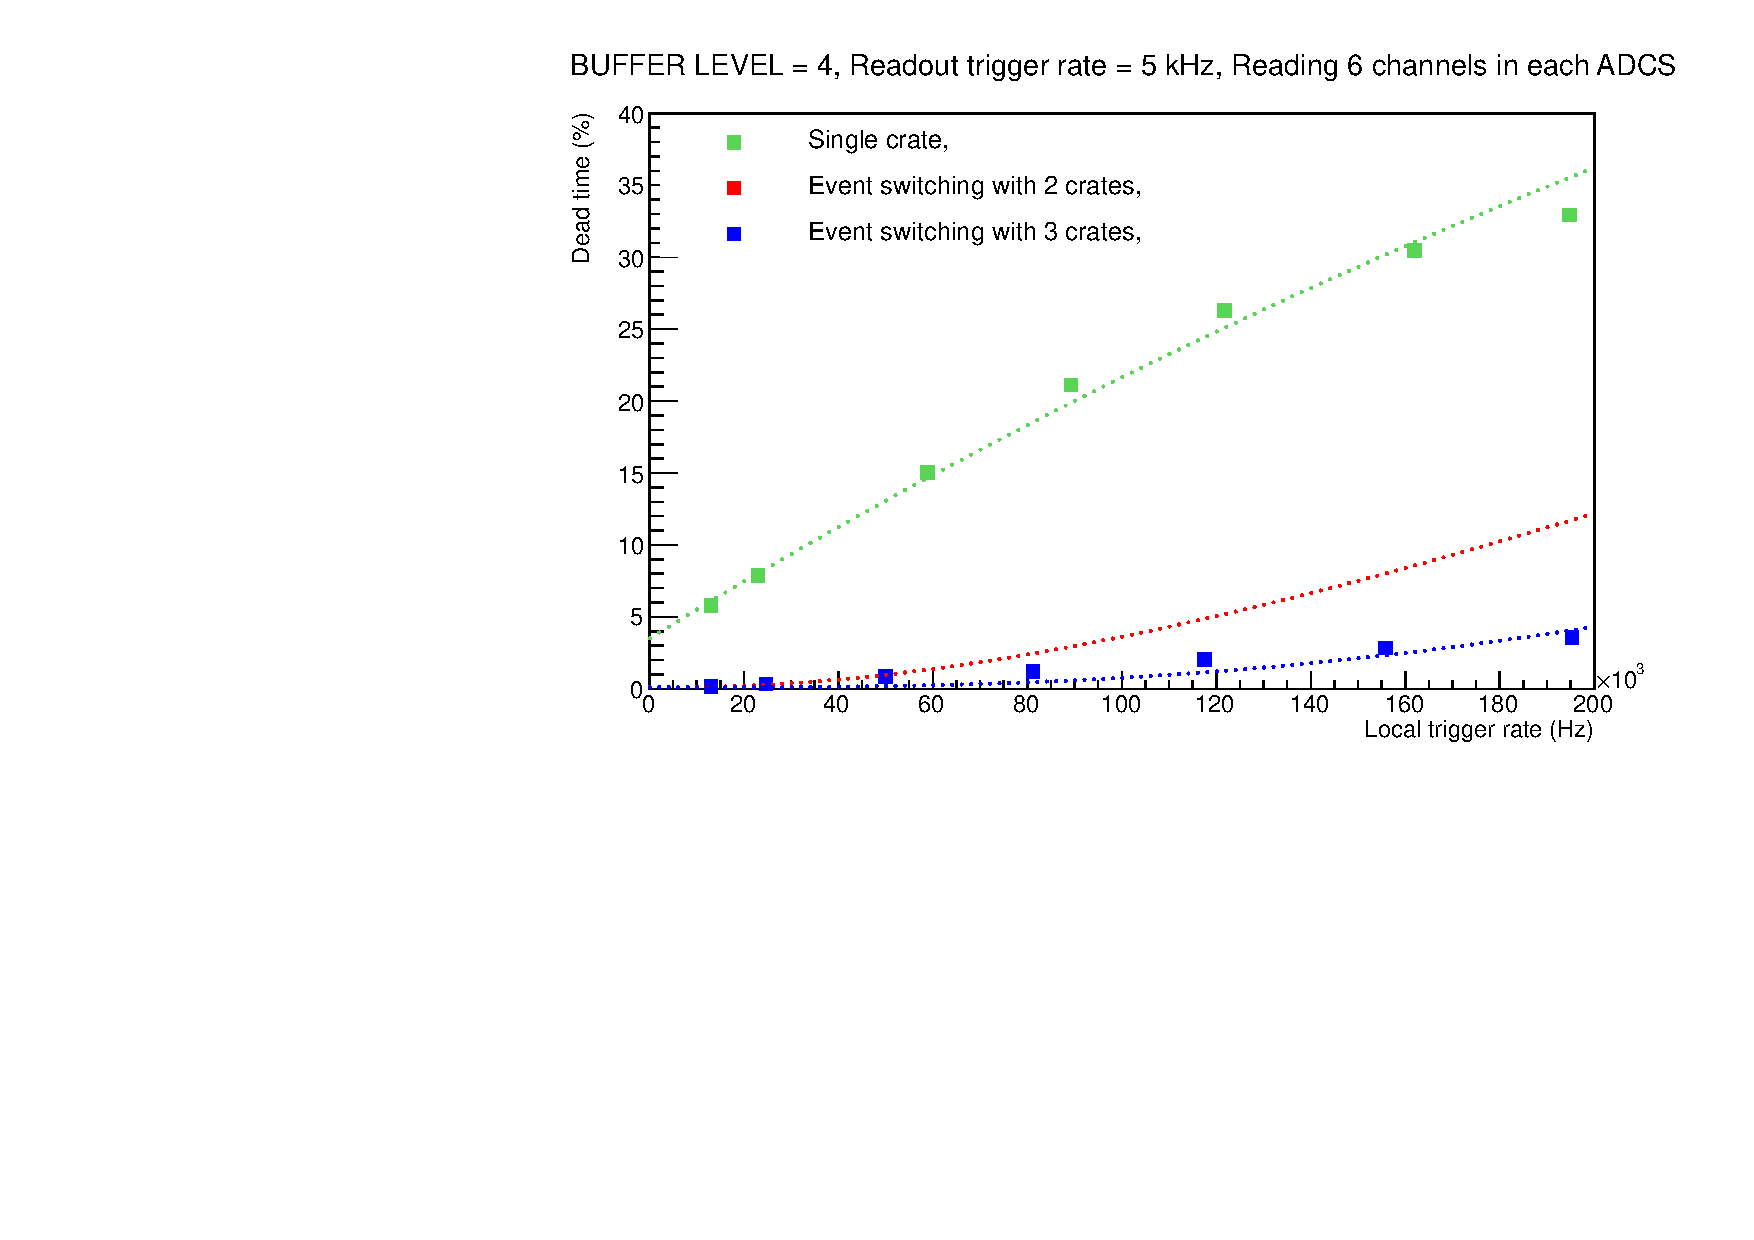
\includegraphics[width=0.75\textwidth]{diffCrate_buffer_4_Readout_5k.pdf}
\end{center}
\caption{Dead time comparison of a single crate system and the event switching mode at Readout trigger rate = 5 kHz. The colored dotted-lines (data) represent the dead time calculated by the model (measured) at BUFFER LEVEL = 4.}
\label{fig:diffCrate_buf4_readout_5}
\end{figure}

Figures~\ref{fig:diffCrate_buf2_local_50} shows the dead time measured and calculated by the dead time model for a single crate and for event switching mode as a function of Readout trigger rate. We can clearly observe that the dead time is reduced significantly even at BUFFER LEVEL = 2. At Readout trigger rate = 5 kHz, the dead time is improved by factor of 3 by event switching, however, this improvement slightly reduces as the contribution of readout busy time increases. Also note that the number of FB crates used in the event switching has no significant effect at Local trigger rate = 50 kHz. 

Figures~\ref{fig:diffCrate_buf4_readout_5} compares the dead time measured for a single crate and for event switching as a function of Local Trigger rate. Here, dead times were measured at Readout trigger rate = 5 kHz and BUFFER LEVEL = 4. The dead time is remarkably improved by event switching and even shows a notable improvement  when an additional FB crate add in to the system, at higher Local rates. 

\section{Conclusion}
Event switching clearly makes a significant improvement in the dead time of the FB system at buffered mode. At Readout trigger rate = 5 kHz and Local trigger rate = 200 kHz (i.e at the expected trigger rates of GEp(5)), the comparison of the dead time of the single crate to the event switching mode can be approximately given by 
\begin{equation}
DT_n = {DT_1}^n
\end{equation}
where $DT_1$ is the dead time obtains by a single crate and $DT_n$ is the dead time obtains at event switching mode by using $n$ number of FB crates.
\end{document}




